\documentclass[12pt, letterpaper]{article}

\usepackage{graphicx}

\title{The \LaTeX{} Document of All Time}
\author{Jay Shen}
\date{October 2024}

\begin{document}

\maketitle

\section{A wild graph appears!}
\subsection{The plot thickens}

\begin{figure}[h]
    \centering
    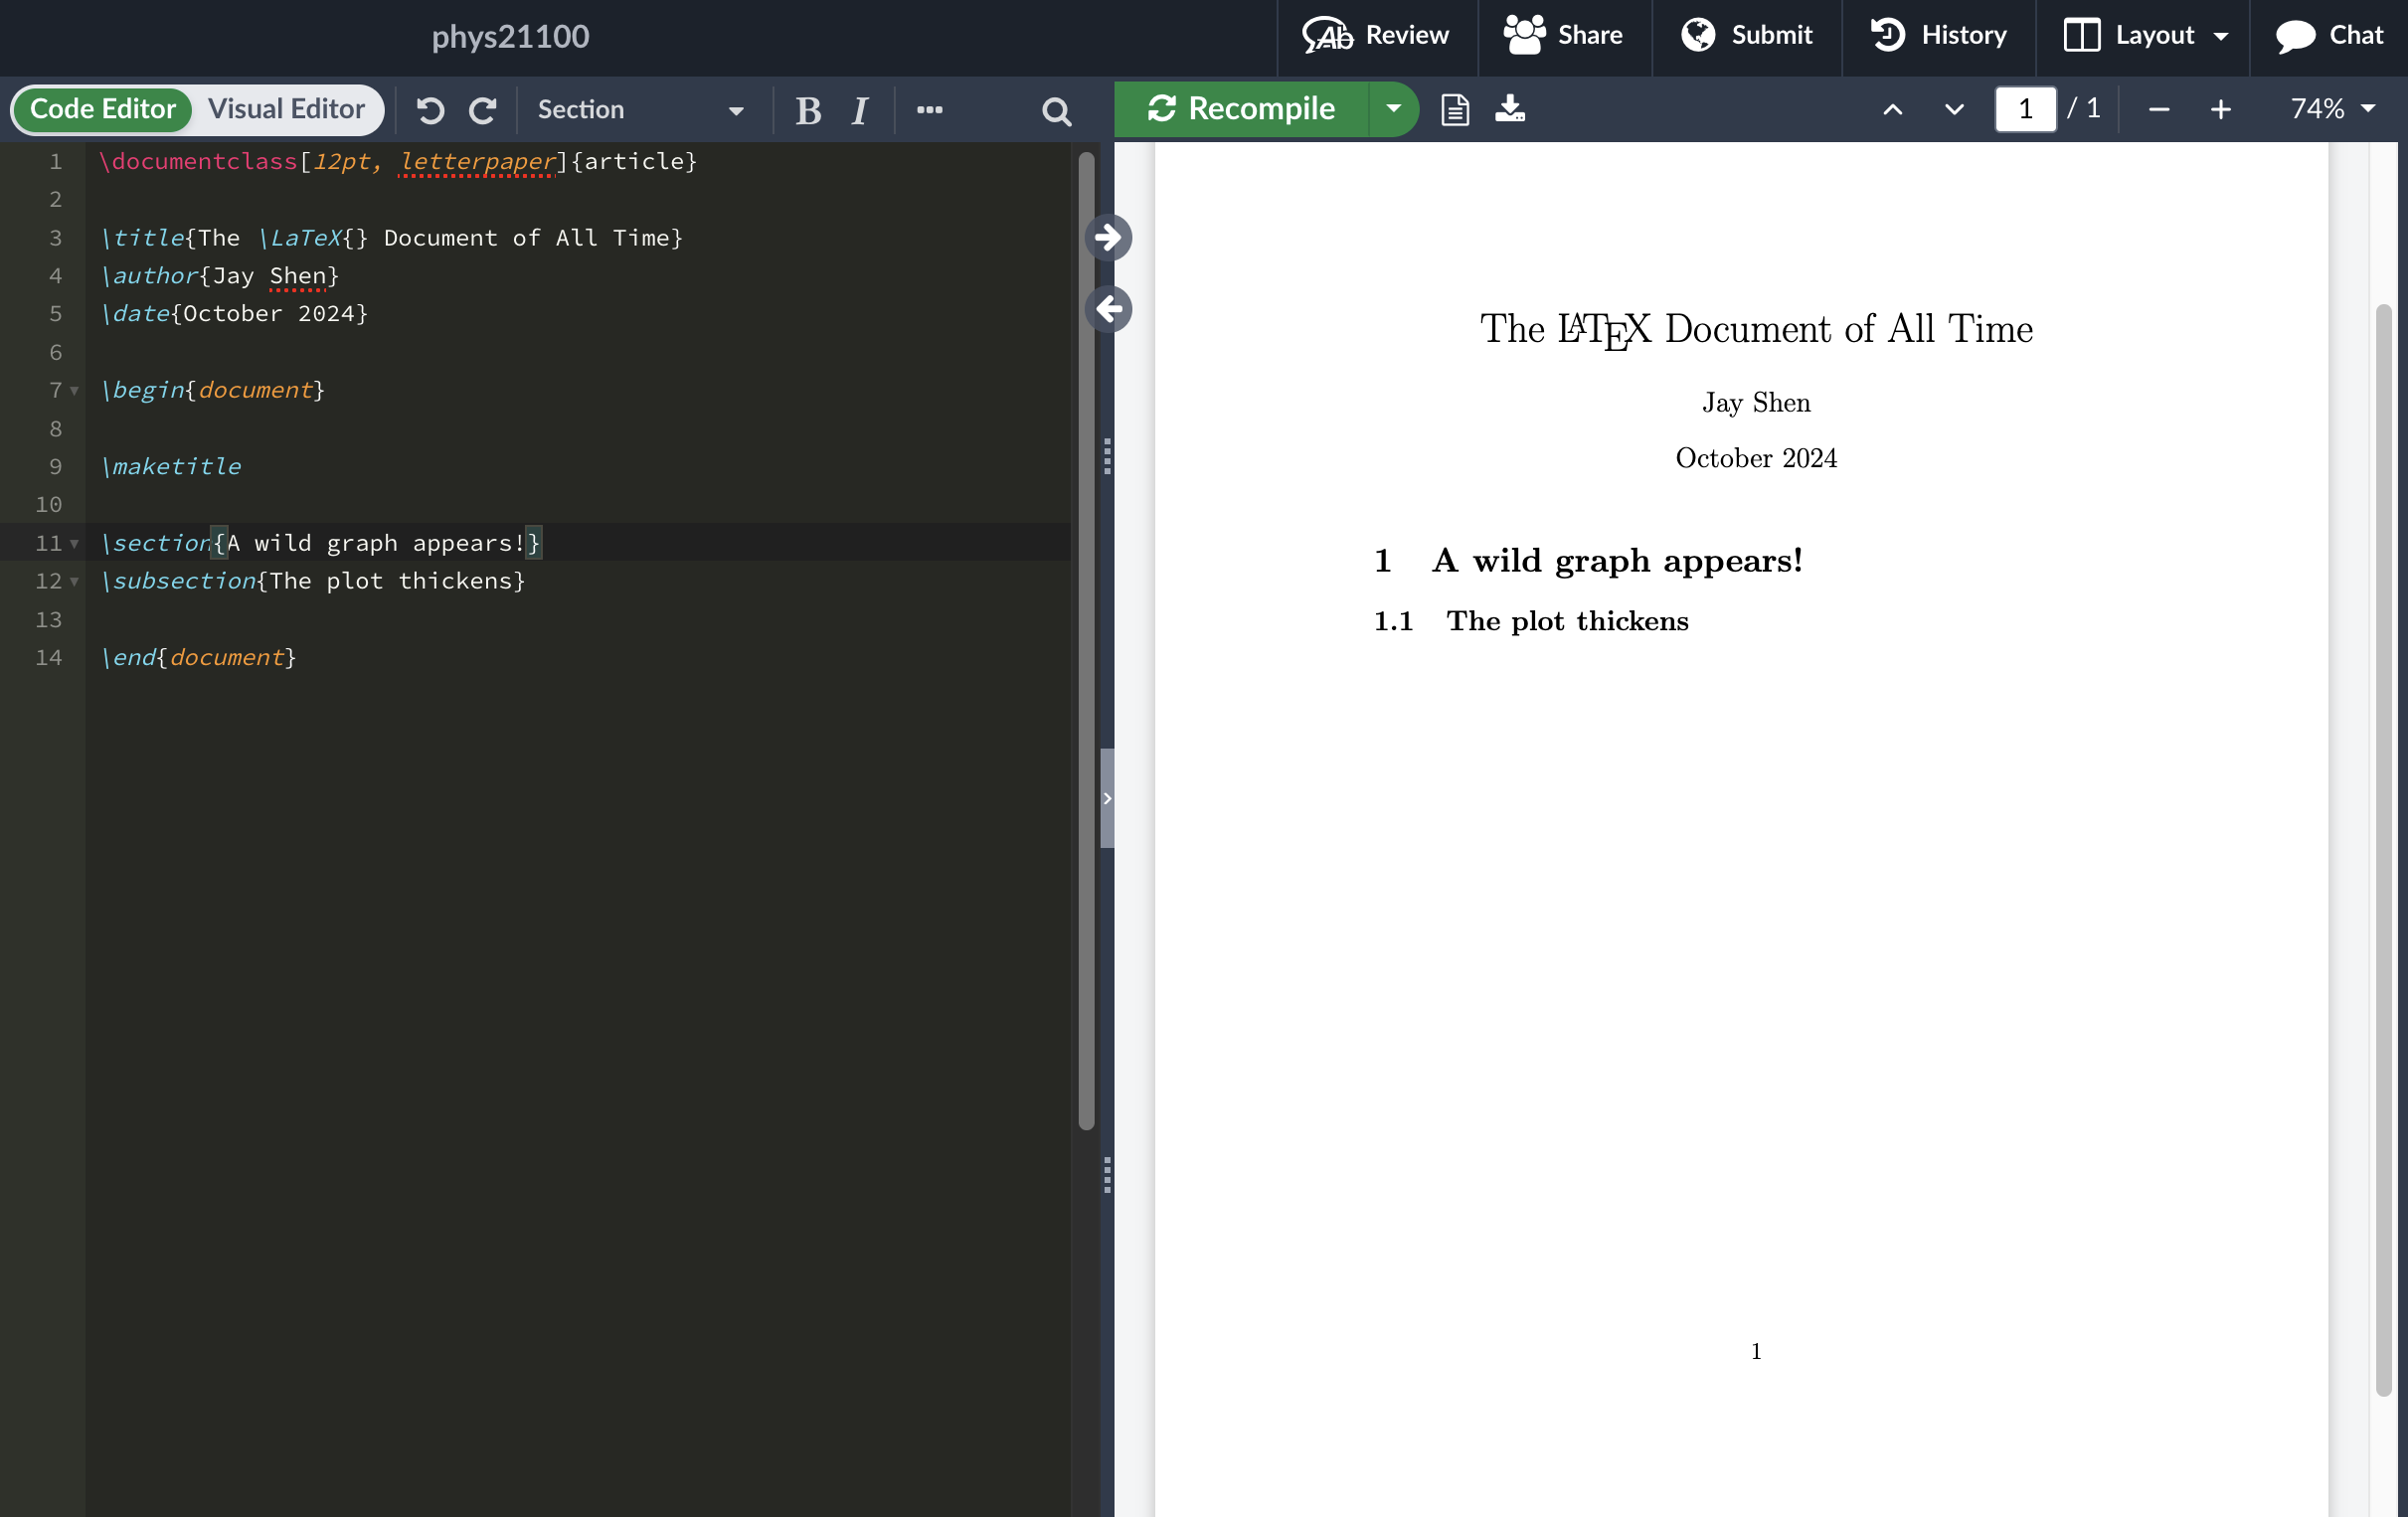
\includegraphics[width=0.75\textwidth]{experiment1/latex_tutorial/image1.png}
    \caption{My Overleaf screen right now. }
    \label{fig:image1}
\end{figure}

I just referenced the hell out of Figure \ref{fig:image1}. 

\section{Why seven ate nine}

Woah, look at this $\rightarrow \hbar$. 
\\
Seven ate nine because 9 is $3^2$. 
Ha ha. 

Fun fact:

\begin{equation} \label{eq:equation1}
    \int^1_0 1 dx = 1
\end{equation}

Equation \ref{eq:equation1} is no longer label-less thanks to me. 

\section{Your table is right this way}

\begin{table}[h!]
\centering
\begin{tabular}{|c c c c|} 
    \hline
    \textbf{A} & \textbf{B} & \textbf{C} & \textbf{D} \\
    \hline
    1 & 2 & 3 & 4 \\ 
    5 & 6 & 7 & 8 \\
    \hline
\end{tabular}
\caption{Nice table dude. }
\label{table:1}
\end{table}

Table \ref{table:1} has been blessed with its very own label. 
I'm a goddamn labeling machine. 

\end{document}